% Paper 2 skeleton (10 Oct 2026). Plan of record: docs/paper2-outline.md.
% Build: pdflatex main && bibtex main && pdflatex main && pdflatex main
% Tables come from paper2/make_tables.py and figures from paper2/make_figures.py; regenerate,
% never edit by hand. Grey \note{} blocks mark the claim and evidence each passage must carry;
% the author replaces each with prose. Venue style: ICML 2027 when its style file is released;
% the NeurIPS preprint style stands in until then.
\documentclass{article}
\usepackage[preprint]{styles/neurips_2026}

\usepackage[utf8]{inputenc}
\usepackage[T1]{fontenc}
\usepackage{hyperref}
\usepackage{url}
\usepackage{booktabs}
\usepackage{amsfonts}
\usepackage{amsmath}
\usepackage{microtype}
\usepackage{graphicx}
\usepackage{xcolor}
\usepackage{natbib}
\graphicspath{{figures/}}

\newcommand{\pyes}{P(\textup{\textsc{yes}})}
\newcommand{\yes}{\textup{\textsc{yes}}}
\newcommand{\note}[1]{\textcolor{gray}{\small\textsl{[#1]}}}

\title{Auditing the Instrument: What Concept-Injection Experiments Measure About LLM
Introspection}

\author{Anonymous authors}

\begin{document}
\maketitle

\begin{abstract}
\note{Write last. One sentence each: the paradigm and its three instrument assumptions (the
vector is live, the dose is comparable, the readout reports self-access); the audit, with
controls of known answer and every arm pre-registered; liveness (C1, C2), dose (C4, C8),
readout (C3, C5, C6); the protocol and its release (C7). Not a verdict on introspection.}
\end{abstract}

% ======================================================================
\section{Introduction}
\label{sec:intro}
\note{The paradigm: inject a concept vector, ask the model whether it detects an injected
thought \citep{lindsey2025introspection,macar2026mechanisms}. Three assumptions every such result
rests on, none checked in the literature. What the paper does: an audit of the instrument, not
a verdict on introspection. Contributions C1--C8 from the outline, one line each.}

\note{Positioning in one sentence: five critiques exist
\citep{hahami2025disturbance,lederman2026contentagnostic,singh2026realitycheck,wu2026steerable};
this paper's contribution is the instrument (liveness, dose, health checks), not another
verdict.}

% ======================================================================
\section{Background and related work}
\label{sec:related}
\note{Outline \S3 table, as prose. Detection results and the defended mechanism
\citep{lindsey2025introspection,macar2026mechanisms}. Content-agnostic and input-editing
critiques \citep{lederman2026contentagnostic,singh2026realitycheck}. The global affirmative
shift \citep{hahami2025disturbance} (C8 tests it). Cross-scale dose confounds and the
residual-norm fix \citep{wu2026steerable} (C4 shows the fix does not transfer). Steerability
predictors \citep{billa2026predicting,braun2025unreliability,bas2025whatcan} (C1 tests them as
health checks). Trained detection \citep{fonsecarivera2025awareness,hahami2026ift} is a
different object.}

% ======================================================================
\section{The audit protocol}
\label{sec:protocol}
\note{Models: Qwen2.5-3B/7B, Gemma-3-4B/12B/27B, Gemma-2-2B for A-F1. Recipes: concept token,
template tail, sentence mean, released. Controls: norm-matched random, impact-matched random,
shuffled, span. Doses: fraction of residual norm, KL-calibrated grid, released raw strengths.
Readouts: steering gate (rule-scored), first-token \pyes{}, rule-scored text. Live rule: steered
at the gate dose and not at dose 0. Every arm pre-registered; amendments and deviations in
Appendix~\ref{app:deviations}. Hardware: free T4s, 4-bit for 12B and 27B.}

% ======================================================================
\section{Results}
\label{sec:results}

\subsection{Liveness, and the checks that should catch it}
\label{sec:liveness}
\note{C1 and C2. Whether a vector steers at all depends on model and read position: template-tail
vectors are inert on Qwen and on the KL-calibrated grid, but the released recipe at its
released strength is live on Gemma-3-27B (Table~\ref{tab:liveness}). No standard health check
finds the live vectors on every model; raw norm runs below chance in four of five sessions;
distinctness is a partial signal; logit-lens accessibility is the first check that works on
three of four sessions, but within one recipe it ranges 0.37--0.82, so it is a screen, not a
certificate (Table~\ref{tab:health}, Figure~\ref{fig:health}).}

\begin{table}[t]
\centering
\small
% Generated by paper2/make_tables.py; do not edit by hand.
\begin{tabular}{llccc}
\toprule
model & study & concept token & template tail & sentence mean \\
\midrule
Qwen2.5-3B & S-2 & 16/30 & 4/30 & 14/30 \\
Qwen2.5-7B & S-2 & 12/30 & 3/30 & 17/30 \\
Gemma-3-4B (KL grid) & S-2 & 3/30 & 2/30 & 4/30 \\
Gemma-3-12B (4-bit) & S-1 & 8/30 & 6/30 & 15/30 \\
Gemma-3-27B (4-bit) & S-1 & 0/30 & 2/30 & 1/30 \\
Gemma-3-27B, released recipe and strength 4 & S-1M & --- & 24/30 & --- \\
\bottomrule
\end{tabular}

\caption{\note{Live vectors per recipe at each session's gate dose (steered at the gate, not at
dose 0), and the released recipe at its released strength.}}
\label{tab:liveness}
\end{table}

\begin{table}[t]
\centering
\resizebox{\linewidth}{!}{% Generated by paper2/make_tables.py; do not edit by hand.
\begin{tabular}{lccccccc}
\toprule
model (live) & norm & distinctness & stability & probe & logit steering & P(YES) shift & logit-lens accessibility \\
\midrule
Qwen2.5-3B (34/90) & 0.56 [0.44, 0.68] & 0.78 [0.68, 0.88] & 0.61 [0.50, 0.73] & 0.61 [0.55, 0.66] & 0.70 [0.59, 0.80] & 0.37 [0.25, 0.49] & 0.69 [0.58, 0.80] \\
Qwen2.5-7B (32/90) & 0.38 [0.26, 0.51] & 0.82 [0.73, 0.90] & 0.61 [0.49, 0.72] & 0.64 [0.59, 0.70] & 0.62 [0.51, 0.74] & 0.35 [0.24, 0.47] & 0.77 [0.66, 0.86] \\
Gemma-3-4B (KL grid) (9/90) & 0.41 [0.21, 0.59] & 0.61 [0.46, 0.75] & 0.52 [0.32, 0.71] & 0.45 [0.29, 0.62] & 0.43 [0.25, 0.64] & 0.54 [0.33, 0.76] & 0.50 [0.28, 0.73] \\
Gemma-3-12B, 4-bit (29/90) & 0.34 & --- & 0.49 & 0.59 & 0.59 & --- & 0.62 [0.50, 0.73] \\
\bottomrule
\end{tabular}
}
\caption{\note{AUC of each health check at telling live from dead vectors, with stratified
bootstrap intervals (none stored for Gemma-3-12B). Logit-lens accessibility is P2-L,
pre-registered before analysis.}}
\label{tab:health}
\end{table}

\begin{figure}[t]
\centering
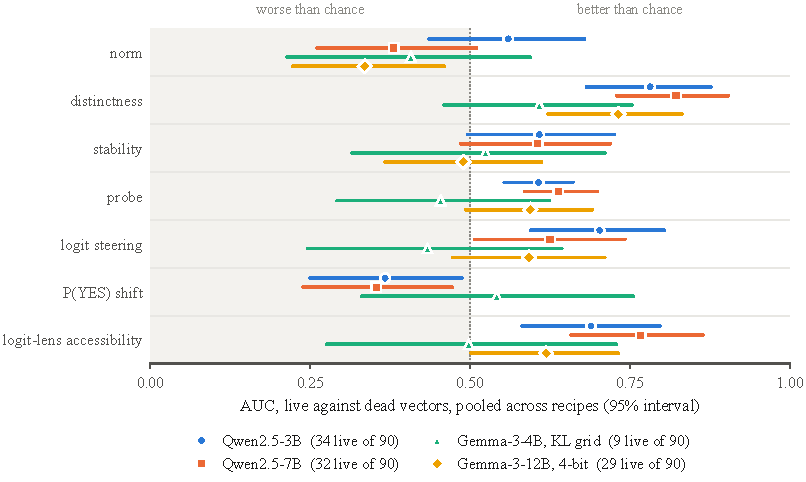
\includegraphics[width=0.6\linewidth]{fig_health_auc}
\caption{\note{Health-check AUCs by model; 0.5 is chance.}}
\label{fig:health}
\end{figure}

\subsection{The inverted \pyes{} check}
\label{sec:inverted}
\note{C3. Where vectors are dead (Qwen), a significant \pyes{} shift predicts a dead vector, not
a live one (AUC 0.367, 0.353). A direct output-steering path explains part of the shift (P2-M,
$\rho$ 0.26, 0.29) but not the inversion (0.367 to 0.388 once removed). The inversion is
framing-specific: dead tail vectors raise introspective \pyes{} by 0.87 at half the residual
norm but factual-NO \pyes{} by only 0.05.}

\subsection{Dose without a unit}
\label{sec:dose}
\note{C4. The same fraction of the residual norm gives next-token KL that differs by over 100x
across families; at the same norm, real vectors move the next token 3--20x less than random
directions on Gemma-3-4B and about 1{,}000x less on 27B; even a vector's own KL does not put models on one curve
(Table~\ref{tab:dose}, Figures~\ref{fig:dosefrac}, \ref{fig:dosekl}, \ref{fig:livekl}). The
released strength sits at about 7 nats, and strength 8 breaks 77\% of generations.}

\begin{table}[t]
\centering
\small
% Generated by paper2/make_tables.py; do not edit by hand.
\begin{tabular}{lccc}
\toprule
fraction of residual norm & 0.25 & 0.5 & 1.0 \\
\midrule
Qwen2.5-3B & 0.00365 & 1.07 & 20.8 \\
Qwen2.5-7B & 0.0896 & 2.56 & 17.4 \\
Gemma-3-4B & 42.9 & 60.4 & 71.3 \\
\bottomrule
\end{tabular}

\medskip

\begin{tabular}{lccc}
\toprule
Gemma-3-4B, KL target (nats) & 0.05 & 0.5 & 5 \\
\midrule
concept KL / random KL & 0.38 & 0.28 & 0.05 \\
\bottomrule
\end{tabular}

\caption{\note{Top: median next-token KL (nats) at the same fraction of the residual norm.
Bottom: on Gemma-3-4B's KL-calibrated grid, real concept vectors' KL over random directions'
KL at each target.}}
\label{tab:dose}
\end{table}

\begin{figure}[t]
\centering
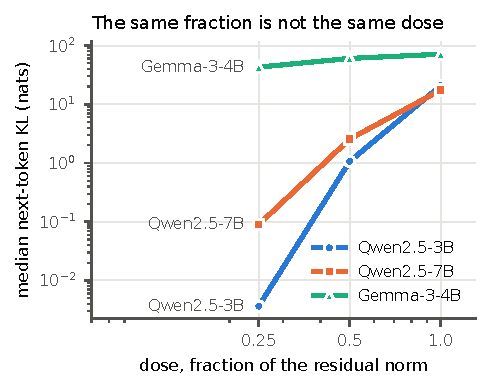
\includegraphics[width=0.48\linewidth]{fig_dose_fraction}\hfill
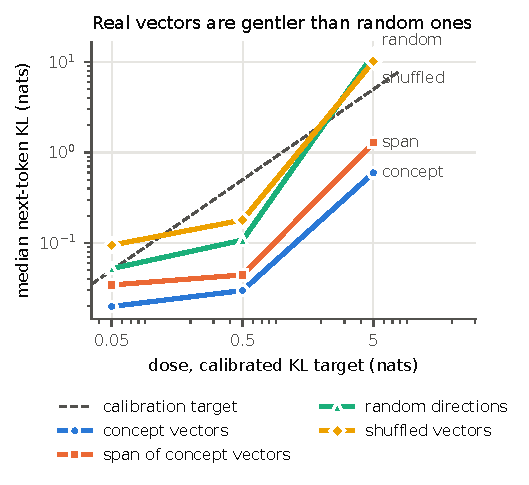
\includegraphics[width=0.48\linewidth]{fig_dose_kl}
\caption{\note{Left: one fraction of the norm, three models. Right: the KL-calibrated grid on
Gemma-3-4B, real and on-manifold vectors against off-manifold ones.}}
\label{fig:dosefrac}
\label{fig:dosekl}
\end{figure}

\begin{figure}[t]
\centering
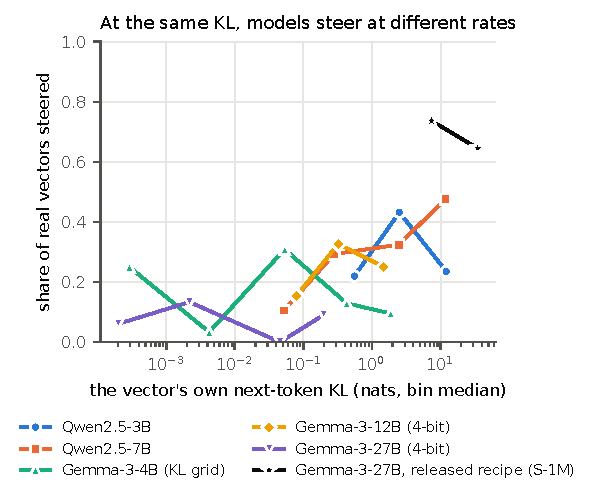
\includegraphics[width=0.6\linewidth]{fig_live_kl}
\caption{\note{Share of real vectors steered against each vector's own next-token KL, by
model (bins of at least 10 vector-doses). Exploratory.}}
\label{fig:livekl}
\end{figure}

\subsection{What detection measures at the published operating point}
\label{sec:operating}
\note{C5 and C8. At the published operating point content-free vectors reproduce the
first-token shift (random 0.305 against real 0.417, $p$ 0.33), and a neutral prompt says
\yes{} 19\% of the time uninjected (S-1M: 0.188 to 0.253). The global yes-bias of
\citet{hahami2025disturbance} is small there (8\% of the introspective rise on Gemma-3-27B at
strength 4; at most 5\% on Qwen-7B at half the norm) and carries 41--67\% only at the highest
doses (Table~\ref{tab:yesbias}, Figure~\ref{fig:yesbias}). Which account is true depends on the
dose, and the dose has no unit (Section~\ref{sec:dose}).}

\begin{table}[t]
\centering
\small
% Generated by paper2/make_tables.py; do not edit by hand.
\begin{tabular}{lllcccc}
\toprule
model & vectors & dose & median KL & introspective & factual-NO & ratio \\
\midrule
Gemma-3-27B & released & strength 4 & 0.000566 & +0.178 & +0.015 & 0.083 \\
Gemma-3-27B & released & strength 8 & 45 & +0.279 & +0.175 & 0.628 \\
Qwen2.5-7B & concept & 0.25 & 2.45e-05 & +0.059 & -0.000 & -0.000 \\
Qwen2.5-7B & concept & 0.5 & 0.0176 & +0.418 & +0.000 & 0.000 \\
Qwen2.5-7B & concept & 1.0 & 30.2 & +0.797 & +0.538 & 0.675 \\
Qwen2.5-7B & tail & 0.25 & 2e-05 & +0.680 & +0.000 & 0.000 \\
Qwen2.5-7B & tail & 0.5 & 0.0119 & +0.866 & +0.046 & 0.054 \\
Qwen2.5-7B & tail & 1.0 & 11.5 & +0.847 & +0.477 & 0.563 \\
Qwen2.5-7B & random & 0.25 & 2.75e-05 & +0.021 & +0.000 & 0.000 \\
Qwen2.5-7B & random & 0.5 & 8.5e-05 & +0.149 & +0.001 & 0.008 \\
Qwen2.5-7B & random & 1.0 & 0.504 & +0.440 & +0.180 & 0.409 \\
\bottomrule
\end{tabular}

\caption{\note{P2-F. Mean \pyes{} change from dose 0, paired by concept: on factual questions
whose answer is NO, and on the introspective question at the same arm and dose. Ratio is
factual-NO over introspective.}}
\label{tab:yesbias}
\end{table}

\begin{figure}[t]
\centering
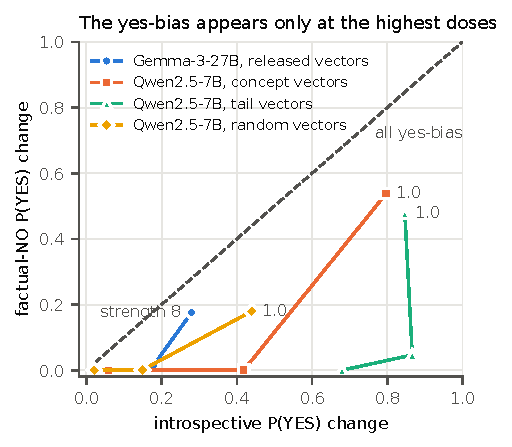
\includegraphics[width=0.55\linewidth]{fig_yesbias}
\caption{\note{Factual-NO against introspective \pyes{} change; the diagonal is a pure yes-bias.}}
\label{fig:yesbias}
\end{figure}

\subsection{The detection rate is a property of the readout}
\label{sec:readout}
\note{C6. Generated-text detection falls from 43\% to 0\% across doses over which the
first-token \pyes{} is flat (about 0.42). Study 3 readout swing; S-4 reanalysis.}

% ======================================================================
\section{A reporting checklist}
\label{sec:checklist}
\note{C7 as practice: a steering gate per vector before any detection number; real-vector KL and
coherence at every dose, with the full dose curve; content-free, impact-matched and span
controls; a neutral framing and a factual-NO control; first-token readouts beside generated text;
never a dose in raw units or fraction of norm alone. Logit-lens accessibility as a cheap screen.}

% ======================================================================
\section{Limitations}
\label{sec:limits}
\note{Free-tier hardware: 4-bit for 12B and 27B; the precision axis is untestable on T4s.
Open models up to 27B, no closed models. 30 concepts. The steering gate is one rule; a stricter
rule belongs in an appendix. No judge-scored numbers. Negative results kept: S-1's criterion,
P2-G, P2-M's secondary.}

\section{Conclusion}
\note{The instrument, not introspection, is what this paper measures; every assumption fails in
some regime and the standard checks do not notice.}

\bibliographystyle{plainnat}
\bibliography{references}

\appendix
\section{Every run, its filing, and every deviation}
\label{app:deviations}
\note{From the notebook and the preregistrations: S-2 (Amendments 1--3), S-1 (Amendments 1--4),
P2-M, P2-F, P2-L, P2-D, P2-G, A-F1, S-11, S-4; dates of filing against dates of data.}

\section{The released code, read}
\note{Template-tail read, unnormalised vectors, strength 4--8, injection from the token before
``Trial'' through generation; normalisation absent in code and not stated in the paper.}

\end{document}
